\section{Theoretical Analysis}
\label{sec:analysis}

In this section, the circuit shown in Figure~\ref{fig:circuit} is analysed
theoretically. This analysis was made with two different methods: the \textbf{Mesh Method} (Subsection \ref{subsec:Mesh Method}) and the \textbf{Node Method} (Subsection \ref{subsec:Node Method}), both based on circuit analysis basic principles:
\begin{itemize}
\item \textbf{Kirchoff Voltage Law (KVL):} This law states that the algebraic sum of all the voltages around any closed loop in a circuit is equal to zero. This means, that the sum of all the potential differences in a closed loop must be zero. This law is directly related with the Energy Conservation principle: if we circulate the loop in one direction, we will end up just where we have started. Therefore, there cannot be any potential difference between the start and the end node, since they are the same node and energy cannot be lost. Notice, that for this assumption to be true, polarities and signs of the elements must be taken in account:$$\sum_{i=1}^{n}V_{i}=0$$
\item \textbf{Kirchoff Current Law (KCL):} This law states that the algebraic sum of all the currents entering a node is equal to algbraic sum of all the currents leaving that same node. This law is also known as the Charge Conservation law: when a current enters a node it as no other option besides leaving the node, since that cannot be any current loss: $$\sum_{i=1}^{n}I_{i}=0$$
  \item \textbf{Ohm's Law:} Ohm's Law states that the current passing through a conductor is propotional to the voltage drop between the two terminals of that conductor: $$V = RI,$$ where $R$ represents the proportionality constant (resistance). 
  
\end{itemize}


\subsection{Mesh Method}
\label{subsec:Mesh Method}
This method consists on assigning currents to the circuit meshes and solving the circuit to find the values of each mesh current, using KVL at each individual mesh that is not connected to any (independent???) current source and Ohm's Law. In doing so we end up with a set of independent equations. In this point, the will be more unknows than equations. So, it is necessary to find more equations in order to have a solvable system. This last equations can be found in the relations between the current sources and the currents assigned to the loops. Now, we can solve the system obtained by using its matricial form. The procedure for this particular circuit is shown bellow:\par
Assuming the currents representend in Figure \ref{fig:MeshMethod}:

\begin{figure}[h] \centering
  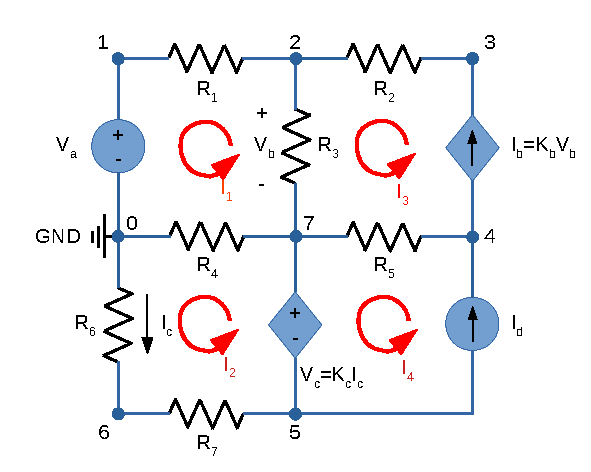
\includegraphics[width=0.7\linewidth]{MeshMethod.pdf}
  \caption{Mesh Currents Identification}
  \label{fig:MeshMethod}
\end{figure}

$$
\begin{cases}
  \text{Mesh 1: } R_{1}I_{1}+V_{a}+R_{4}(I_{1}-I_{2})+R_{3}(I_{1}-I_{3}) = 0\\
  \text{Mesh 2: } R_{4}(I_{2}-I_{1})+R_{6}I_{2}+R_{7}I_{2}-K_{c}I_{2} = 0\\
  \text{Current b: } I_{3} = I_{b} = K_{b}V_{b}\\
  \text{Current d: } I_{4} = I_{d}\\
  \\
  \text{Ohm's Law: } V_{b} = R_{3}(I_{3}-I_{1})
\end{cases}
$$

$$
\begin{bmatrix}
  R_{1}+R_{3}+R_{4} & -R_{4} & -R_{3} & 0 \\
  -R_{4} & R_{4}+R_{6}+R_{7}-K_{c} & 0 & 0\\
  R_{3}K_{b} & 0 & 1-K_{b}R_{3} & 0\\
  0 & 0 & 0 & 1
\end{bmatrix}
=
\begin{bmatrix}
  I_{1}\\
  I_{2}\\
  I_{3}\\
  I_{4}
\end{bmatrix}
\begin{bmatrix}
  -V_{a}\\
  0\\
  0\\
  I_{d}
\end{bmatrix}
$$

\subsection{Node Method}
\label{subsec:Node Method}


\subsection{Theoretical Analysis Results}
\begin{table} [H]
  \centering
  \begin{tabular}{|l|r|}
    \hline    
    {\bf Name} & {\bf Value [A or V]} \\ \hline
    I_b & -0.000226\\ \hline
I_d & 0.001012\\ \hline
I_{R1} & 0.000216\\ \hline
I_{R2} & -0.000226\\ \hline
I_{R3} & -0.000010\\ \hline
I_{R4} & 0.001195\\ \hline
I_{R5} & -0.001238\\ \hline
I_{R6} & 0.000978\\ \hline
I_{R7} & 0.000978\\ \hline
V_1 & 5.125627\\ \hline
V_2 & 4.903891\\ \hline
V_3 & 4.446215\\ \hline
V_4 & 8.768409\\ \hline
V_5 & -2.982745\\ \hline
V_6 & -1.975719\\ \hline
V_7 & 4.934963\\ \hline

  \end{tabular}
  \caption{Operating point. A variable preceded by @ is of type {\em current}
    and expressed in Ampere; other variables are of type {\it voltage} and expressed in
    Volt.}
  \label{tab:op_analysis}
\end{table}


